\chapter{Planificación}

La planificación del proyecto es una etapa crucial que determina cómo se llevará a cabo el desarrollo del mismo, asegurando que los recursos se utilicen de manera eficiente y que se cumplan los plazos establecidos. En este capítulo, se detallará cómo se ha organizado el proyecto siguiendo los principios ágiles mencionados en el capítulo de metodología. Este capítulo cubre las rúbricas relacionadas con la organización y gestión del tiempo y recursos del proyecto, la estructuración de las tareas y la implementación de herramientas y técnicas para una gestión eficiente. Además, se describirán las estrategias de planificación y el seguimiento del progreso mediante el uso de \textit{issues} y \textit{milestones}.

\section{Organización del proyecto}

Como se ha mencionado anteriormente, el proyecto se organizará y planificará siguiendo un enfoque ágil. Para garantizar la aplicación coherente de estos principios, la memoria se desarrollará iterativa e incrementalmente, con actualizaciones a medida que avanza el proyecto y se toman decisiones. Esto nos permite evaluar continuamente cómo estamos añadiendo valor al proyecto.

\subsection{\textit{Issues}}

A lo largo del proyecto se van a ir encontrando diferentes problemas que se han de resolver. Para llevar un control de los mismos se han ido creando \textit{\textbf{issues}}. 

Los \textit{\textbf{issues}} son fundamentales en el desarrollo ágil, ya que representan problemas identificados durante el ciclo de vida del proyecto. En este contexto, los issues no solo permiten documentar y gestionar incidencias, sino que también aseguran que se avance de manera organizada hacia los hitos o milestones establecidos. Cada \textit{\textbf{issue}} está vinculado a una historia de usuario (HU), lo cual permite una trazabilidad directa entre las necesidades del usuario y las acciones concretas que se realizan para satisfacerlas.

Las HUs definen requisitos específicos desde la perspectiva del usuario, y al desglosarse en \textit{\textbf{issues}}, permiten que cada necesidad se aborde en pequeños incrementos. Esto facilita la adaptación y el ajuste continuo, características clave del enfoque ágil, permitiendo iterar y mejorar continuamente el producto en respuesta al feedback y los cambios en las necesidades del usuario. Esta sección cubre la rúbrica de seguimiento y resolución de problemas de manera organizada y documentada.

\begin{figure}[H]
    \caption{Captura de pantalla del listado de \textit{issues} del repositorio del proyecto de \textit{GitHub}.}
    \centering
    \vspace*{0.5cm}
    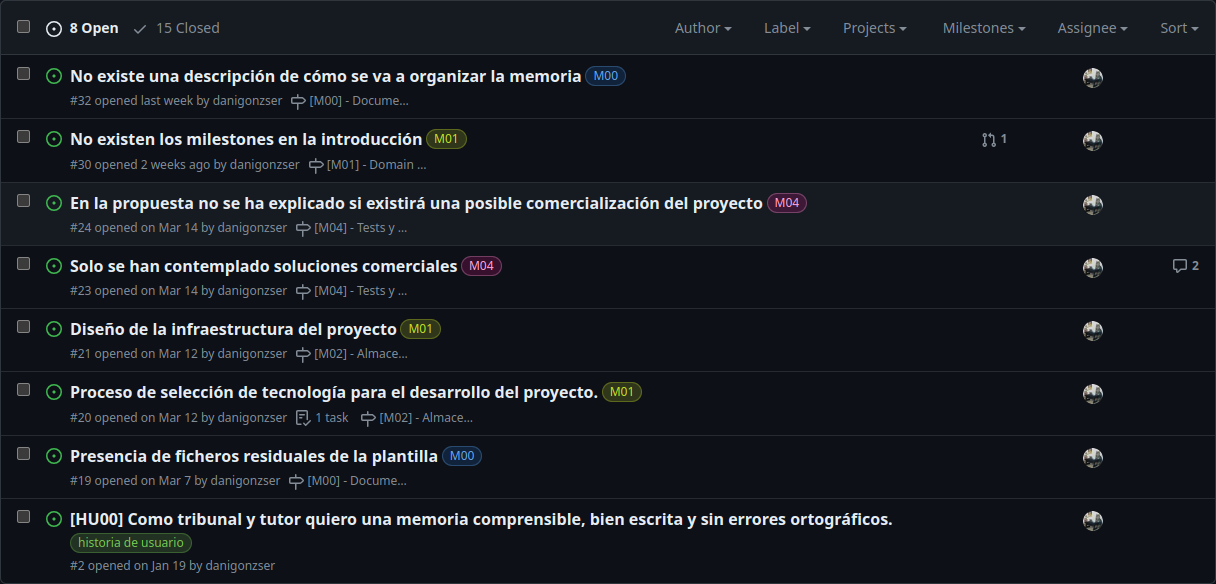
\includegraphics[scale=0.2]{figuras/github_issues.png}
\end{figure}

Existe un acceso a la documentación de la metodología seguida que se puede consultar en el siguiente \href{https://github.com/danigonzser/proyecto-tfg/issues?q=is%3Aissue+is%3Aclosed}{enlace}, aquí se encuentra el registro completo de los \textit{issues} cerrados, que ilustran el proceso de resolución de problemas y la evolución del proyecto. A continuación, se muestra un pantallazo de los \textit{issues} cerrados:

\begin{figure}[H]
    \caption{Pantallazo del listado de issues cerradas.}
    \centering
    \vspace*{0.5cm}
    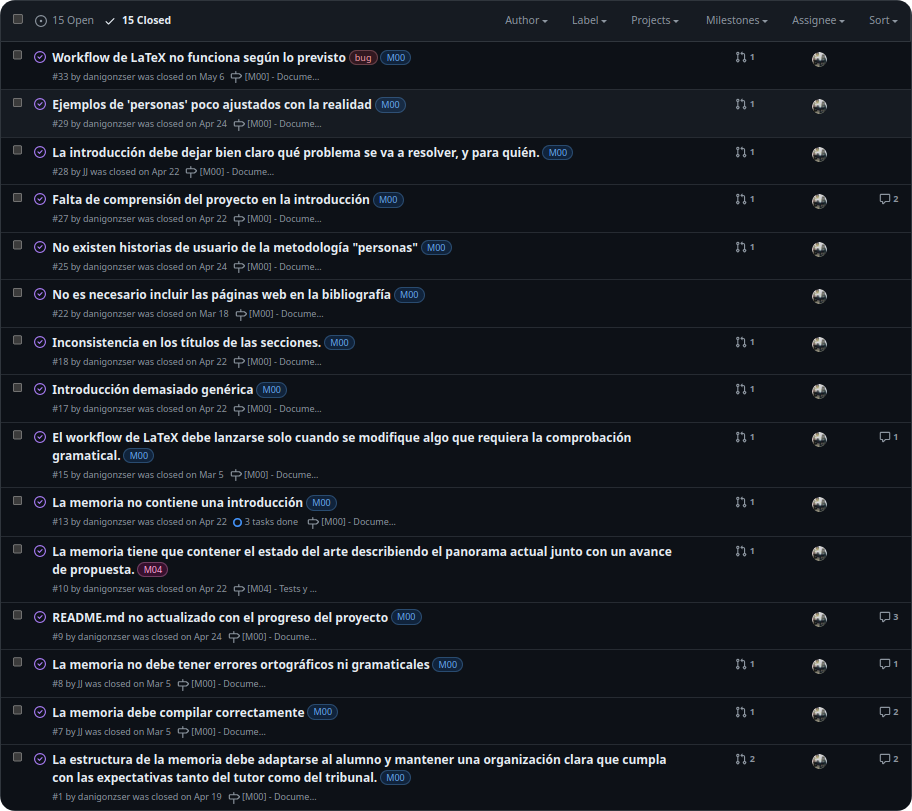
\includegraphics[scale=0.2]{figuras/listado_issues_cerradas.png}\label{fig:figuras/listado_issues_cerradas.png}
\end{figure}

\section{Secuenciación}

La secuenciación de qué hacer en nuestro proyecto se realiza mediante el uso de \textit{milestones} en GitHub, que son el equivalente a los \textit{sprints} en el enfoque ágil. Los \textit{milestones} se han producido a partir de las historias de usuario, asegurando que cada fase del proyecto esté orientada a cumplir con las necesidades y expectativas del usuario final. Un conjunto específico de \textit{issues} puede ser incluido en un \textit{milestone} y, al finalizar el \textit{sprint}, estos \textit{issues} deben estar resueltos. Al concluir el \textit{milestone}, debe resultar en un producto mínimamente viable y en nuestro repositorio vamos a etiquetarlos como nueva versión del proyecto.

\subsection{Milestones}

\begin{itemize}
    \item \textbf{[M00] \- Estructuración inicial del proyecto}
    \begin{itemize}
        \item \textit{Descripción}: Este \textit{milestone} abarca la creación de la documentación inicial, la planificación del proyecto y la configuración de las herramientas necesarias. Esta parte de la memoria inicial es esencial para establecer una base sólida para el desarrollo del proyecto, para la entrega continua y la colaboración.
    \end{itemize}

    \item \textbf{[M01] \- Modelo del problema}
    \begin{itemize}
        \item \textit{Descripción}: Mediante el DDD se va a realizar un análisis del problema que permita obtener una comprensión profunda de todo el contexto del negocio y de la estructura del software.
    \end{itemize}
\end{itemize}

A partir de aquí, los \textit{milestones} se irán definiendo y ajustando conforme avance el proyecto, siguiendo los principios del desarrollo ágil que promueven la adaptación continua y la respuesta al cambio. Los \textit{milestones} sucesivos se centrarán en la implementación, cubriendo las rúbricas de seguimiento de hitos y entregables, así como la capacidad de respuesta a nuevos desafíos y requerimientos del proyecto.
